\section{Benchmarks of the ACE algorithm}
\label{sec:ace-benchmarks}

The preceding sections established the theory and representation of a process tensor, and showed how the same \texttt{ProcessTensor} can be interrogated with different instruments and testers.
We now map the practical performance of its ACE constructor: how time-discretisation errors scale, how the timestep and cutoff affect PT-MPO compressibility, and how the implementation performs against the original C++ ACE toolkit.

All data are generated by scripts in the \texttt{benchmark/} directory in the main repository.
Unless stated otherwise, both the system and mode-combination steps use second-order Trotterisation.
We use \texttt{Paanini}, an AMD Ryzen Threadripper 7980X workstation with 64 physical cores, 128 hardware threads, 256~GiB RAM, and running on Ubuntu 22.04.5 to run all of our benchmarks in this section.


%%%%%%%%%%%%%%%%%%%%%%%%%%%%%%%%%%%%%%%%%%%%%%%%%%%%%%%%%%%%%%%%%%%%%%%%%%%
\subsection{Correctness and discretisation errors}
\label{subsec:ace-correctness}

Our validation model is a single spin coupled to four independent bath spins,
%
\begin{equation}
    H=S_x^{(S)}+\sum_{m=1}^{4}
    \left[\omega_m S_x^{(B_m)}
    +g_m S_z^{(B_m)}S_z^{(S)}\right],
    \quad \omega_m=0.5+0.1m,\quad g_m=0.2+0.3m ,
    \label{eq:ace-validation-hamiltonian}
\end{equation}
%
with \(\hbar=1\), \(S_\alpha=\sigma_\alpha/2\), and all spins initially in \(\lvert\uparrow\rangle\).
The joint Hilbert space has dimension \(2^5=32\), allowing direct diagonalisation without timestep discretisation to provide the reference trajectory.

%
\begin{figure*}[h]
    \centering
    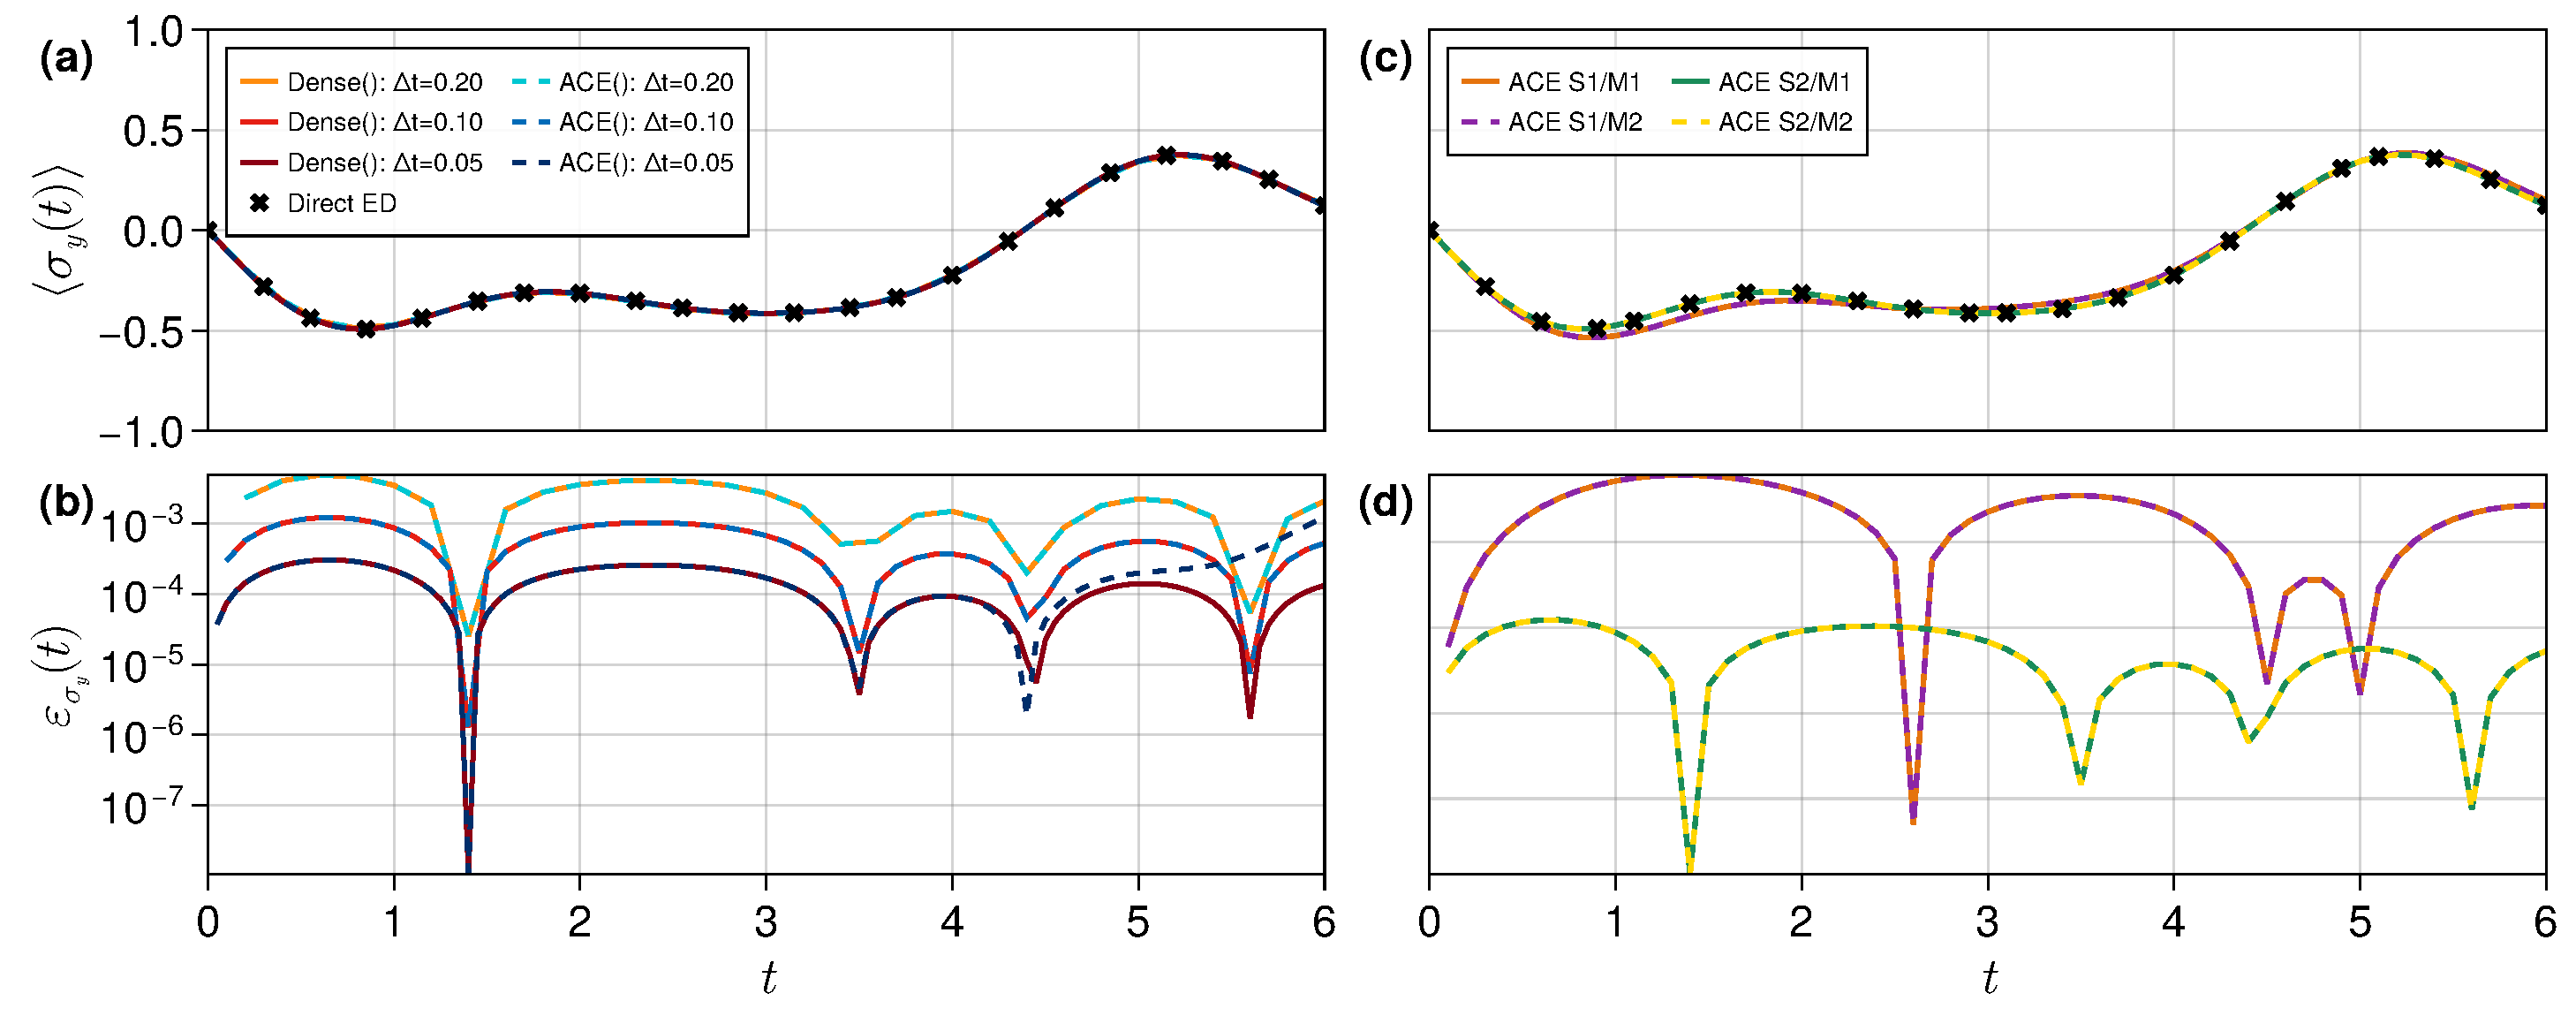
\includegraphics[width=0.98\textwidth]{figures/ace_correctness.pdf}
    \caption{Correctness and propagation errors for the four-mode spin bath.
    Panel (a) shows the system-spin observable $\langle\sigma_y(t)\rangle$ from direct ED, uncompressed \texttt{Dense()}, and \texttt{ACE()} for three different $\Delta t$ values; panel (b) shows their absolute errors relative to ED.
    Panels (c,d) compare first- and second-order system and mode-combination splittings at fixed $\Delta t$.}
    \label{fig:ace-correctness}
\end{figure*}
%

Figure~\ref{fig:ace-correctness} compares direct system--environment evolution with uncompressed \texttt{Dense()} and compressed \texttt{ACE()} process tensors for $\Delta t=0.20$, $0.10$, and $0.05$.
The plotted observable is the transverse system-spin polarisation $\langle\sigma_y(t)\rangle$, evaluated from the reduced state as $\operatorname{Tr}[\sigma_y\rho_S(t)]$.
The compressed tensors are constructed with \texttt{ACE(cutoff=1e-12, compression=:canonzip)}.
We define
%
\begin{equation}
    \varepsilon_{\sigma_y}(t)=
    \left|\langle\sigma_y(t)\rangle_{\rm method}
    -\langle\sigma_y(t)\rangle_{\rm ED}\right|.
    \label{eq:ace-observable-error}
\end{equation}
%
In panel (a), the \texttt{Dense()} and \texttt{ACE()} trajectories lie on top of one another and closely follow the discretisation-free ED result.
Panel (b) resolves the remaining timestep error: the error curves shift systematically downward as $\Delta t$ is reduced from $0.20$ to $0.10$ and then to $0.05$.
The near coincidence of the \texttt{Dense()} and \texttt{ACE()} errors at each timestep shows that compression at the stated cutoff adds no visible error on this scale; the observed convergence towards ED is instead controlled by the time discretisation and propagation splitting.

At fixed $\Delta t=0.10$, panels (c) and (d) separate the two Trotter choices made during an ACE construction.
The labels S1 and S2 refer to the system--environment splitting in Eq.~\eqref{eq:system-bath-splitting}: S1 applies the environmental and free-system maps in an asymmetric first-order sequence, whereas S2 places half of the free-system evolution on either side of the environmental map to give the symmetric second-order sequence.
The labels M1 and M2 make the analogous distinction when the independently propagated mode influences of Eq.~\eqref{eq:ace-independent-mode-decomposition} are combined: M1 joins them in a first-order ordered product, while M2 uses a symmetric second-order composition before the SVD compression in Eq.~\eqref{eq:ace-sequential-update}.
For this particular four-spin bath the mode generators commute, so changing M1 to M2 leaves the result unchanged; the visible improvement comes from replacing S1 by S2.

In general, the error in an observable will stem from four sources:
%
\begin{equation}
    \varepsilon_{\rm obs}\lesssim
    \varepsilon_{\Delta t}
    +\varepsilon_{\rm sys}
    +\varepsilon_{\rm mode}
    +\varepsilon_{\rm SVD}.
\end{equation}
%
Here \(\varepsilon_{\Delta t}\) is the finite-timestep propagation error, \(\varepsilon_{\rm sys}\) and \(\varepsilon_{\rm mode}\) arise from the system--environment and intermode Trotter splittings, and \(\varepsilon_{\rm SVD}\) is introduced by SVD truncation.
For the commuting mode generators used here, \(\varepsilon_{\rm mode}=0\); the observed deviation from ED is therefore set by the remaining contributions, dominated in this converged calculation by the timestep.

%%%%%%%%%%%%%%%%%%%%%%%%%%%%%%%%%%%%%%%%%%%%%%%%%%%%%%%%%%%%%%%%%%%%%%%%%%%
\subsection{Temporal bond dimensions and compressibility}
\label{subsec:ace-bond-dimensions}

For the temporal-bond study we use the unpolarised central-spin model
%
\begin{equation}
    H=\frac{J}{N}\sum_{k=1}^{N}
    (S_xs_k^x+S_ys_k^y+S_zs_k^z),\qquad H_S=H_{B_k}=0 ,
    \label{eq:ace-central-spin}
\end{equation}
%
with the system initially along \(+x\) and independently sampled pure bath-spin states, uniform on the Bloch sphere.
A single archived \texttt{Random.Xoshiro(20260905)} realisation defines the bath orientations for every run.
The sweep uses \(N=50\), \(T=21\), \(\Delta t\in\{1.5,0.5,0.2,0.1,0.05\}\), and \(\epsilon_{\rm SVD}\in\{10^{-6},10^{-8},10^{-10},10^{-12}\}\).

Each internal bond \(\chi_k\) of a PT-MPO crosses the temporal cut at \(t_k=k\Delta t\).
Its dimension \(D_k=\dim(\chi_k)\) counts the effective memory states needed to transmit the influence of the history before that cut to interventions made afterwards.
Inspecting \(D_k\) along the time direction therefore shows where the environmental history is easiest or hardest to compress, rather than reducing the whole process to a single cost estimate.

%
\begin{figure}[h]
    \centering
    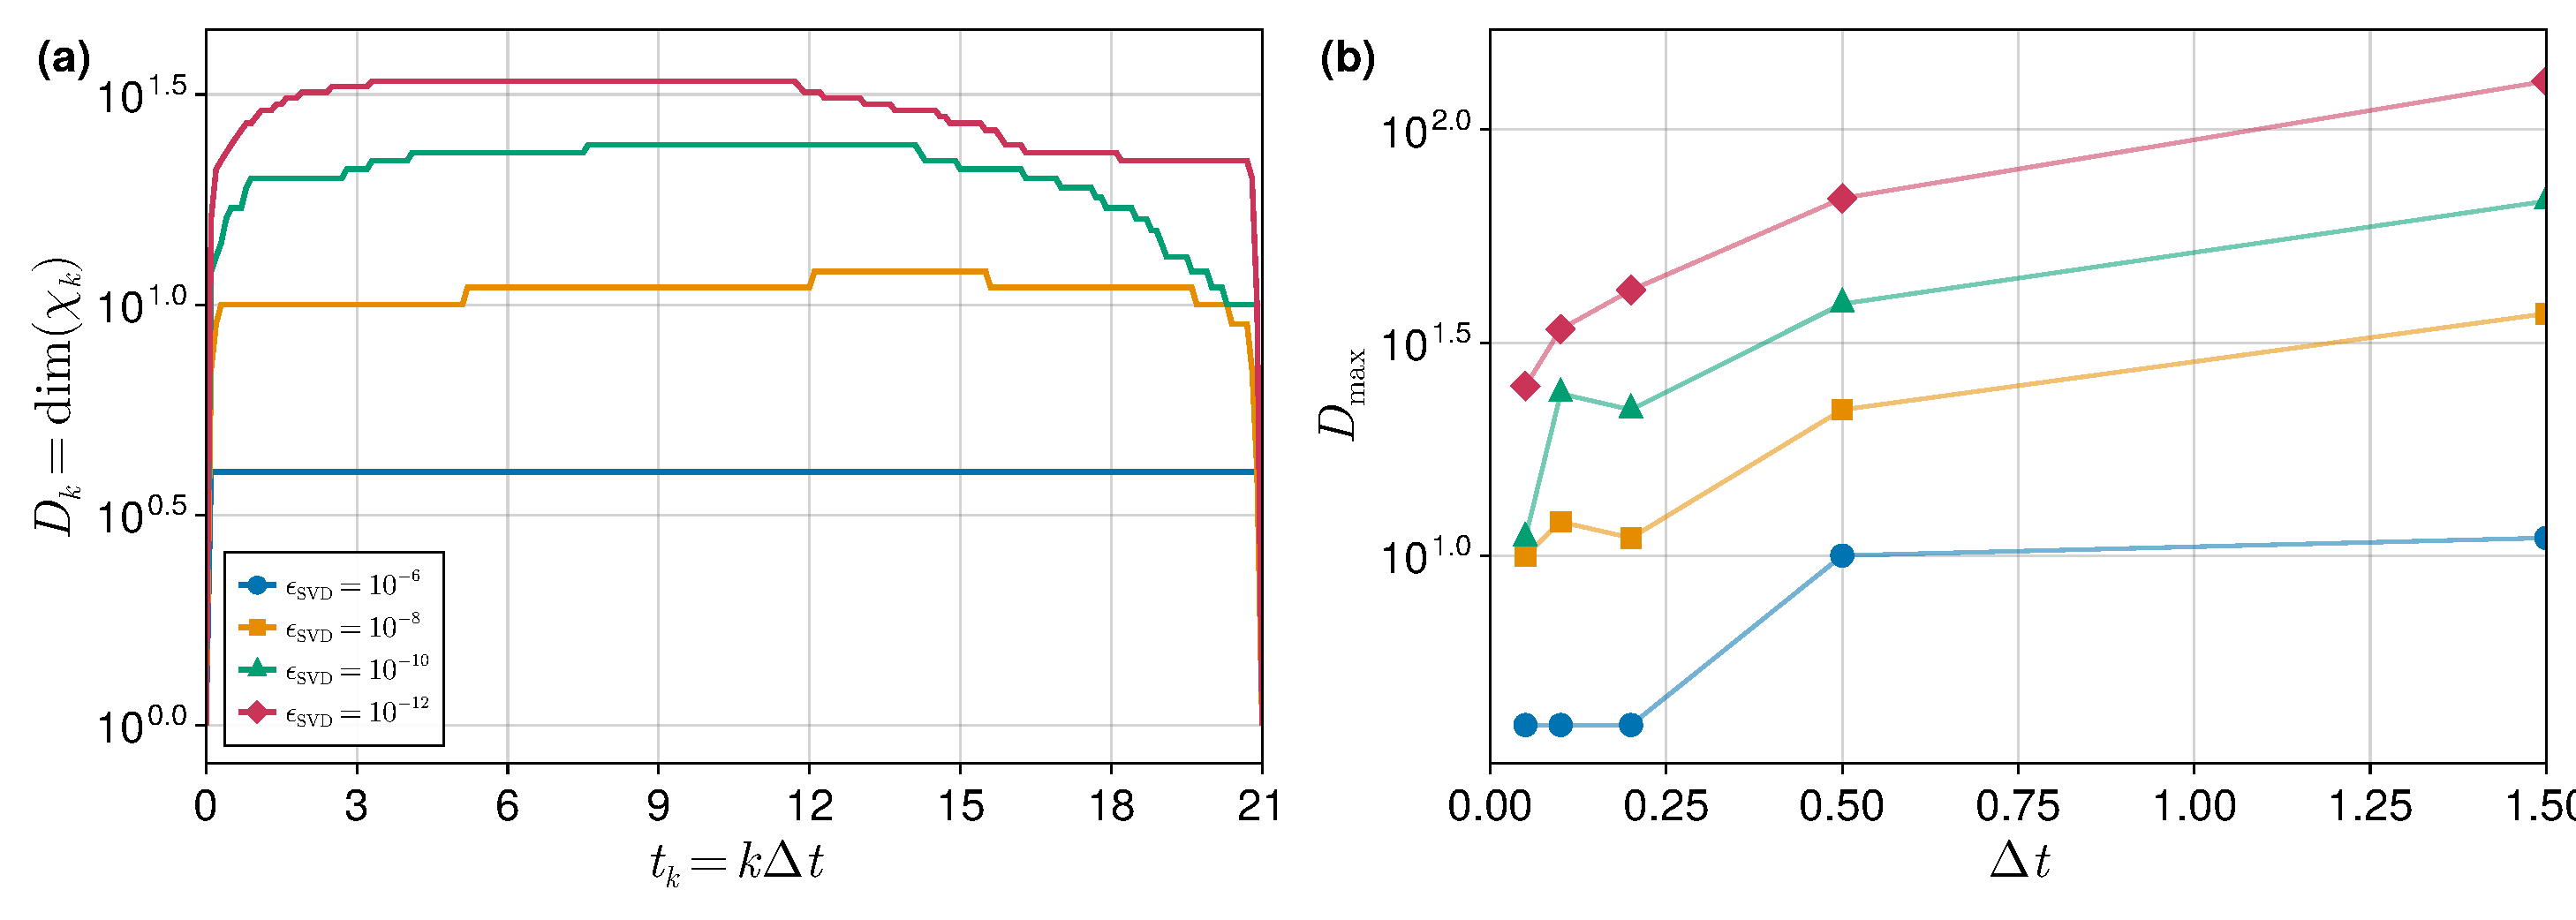
\includegraphics[width=0.98\columnwidth]{figures/ace_temporal_bonds.pdf}
    \caption{Temporal compressibility of the unpolarised central-spin process tensor.
    (a) Internal bond dimensions along the temporal MPO for several relative cutoffs.
    (b) Maximum internal bond dimension versus timestep and cutoff.
    Open symbols indicate runs limited by \texttt{maxdim}; the bath realisation is fixed across all points.}
    \label{fig:ace-bonds}
\end{figure}
%

Figure~\ref{fig:ace-bonds} applies this diagnostic to the unpolarised central-spin model in Eq.~\eqref{eq:ace-central-spin}.
Panel (a) follows \(D_k\) across all internal time legs.
Tightening the relative SVD cutoff retains weaker singular directions at every cut, so the temporal memory spaces become larger and the bond profile rises.
This is the expected accuracy--cost trade-off: a tighter cutoff preserves more channels through which past system--bath correlations can affect the future.

Panel (b) condenses each profile to
%
\begin{equation}
    D_{\max}=\max_{1\leq k\leq n_{\rm steps}-1}D_k ,
    \label{eq:ace-dmax}
\end{equation}
%
excluding the trivial boundary bonds, and compares this maximum across timesteps and cutoffs.
At a fixed cutoff, the observed \(D_{\max}\) increases with \(\Delta t\).
Over a longer interval the system and bath undergo more non-trivial joint dynamics before the next temporal leg is exposed; the resulting one-step influence can explore a larger bath operator subspace and therefore requires more effective memory states to represent.
For smaller \(\Delta t\), each individual step is closer to the identity and typically occupies a simpler subspace, although more PT-MPO cores are needed to reach the same final time.

%%%%%%%%%%%%%%%%%%%%%%%%%%%%%%%%%%%%%%%%%%%%%%%%%%%%%%%%%%%%%%%%%%%%%%%%%%%
\subsection{Compression schedules and accuracy--cost trade-offs}
\label{subsec:ace-compressors}

The central-spin scaling below uses the model of Eq.~\eqref{eq:ace-central-spin}, while the cutoff-versus-error comparison additionally uses a heterogeneous eight-spin environment.
The package currently provides \texttt{:zipup\_cpp} and \texttt{:canonzip} compression schedules.
The former follows the C++ ACE join order: truncation is applied during the forward join and the resulting chain is swept backward.
The latter forms the complete mode join, canonicalises towards the final time, and performs a relative SVD sweep from right to left.
Both use the same cutoff and \texttt{maxdim}; only the schedule differs.

%
\begin{figure*}[h]
    \centering
    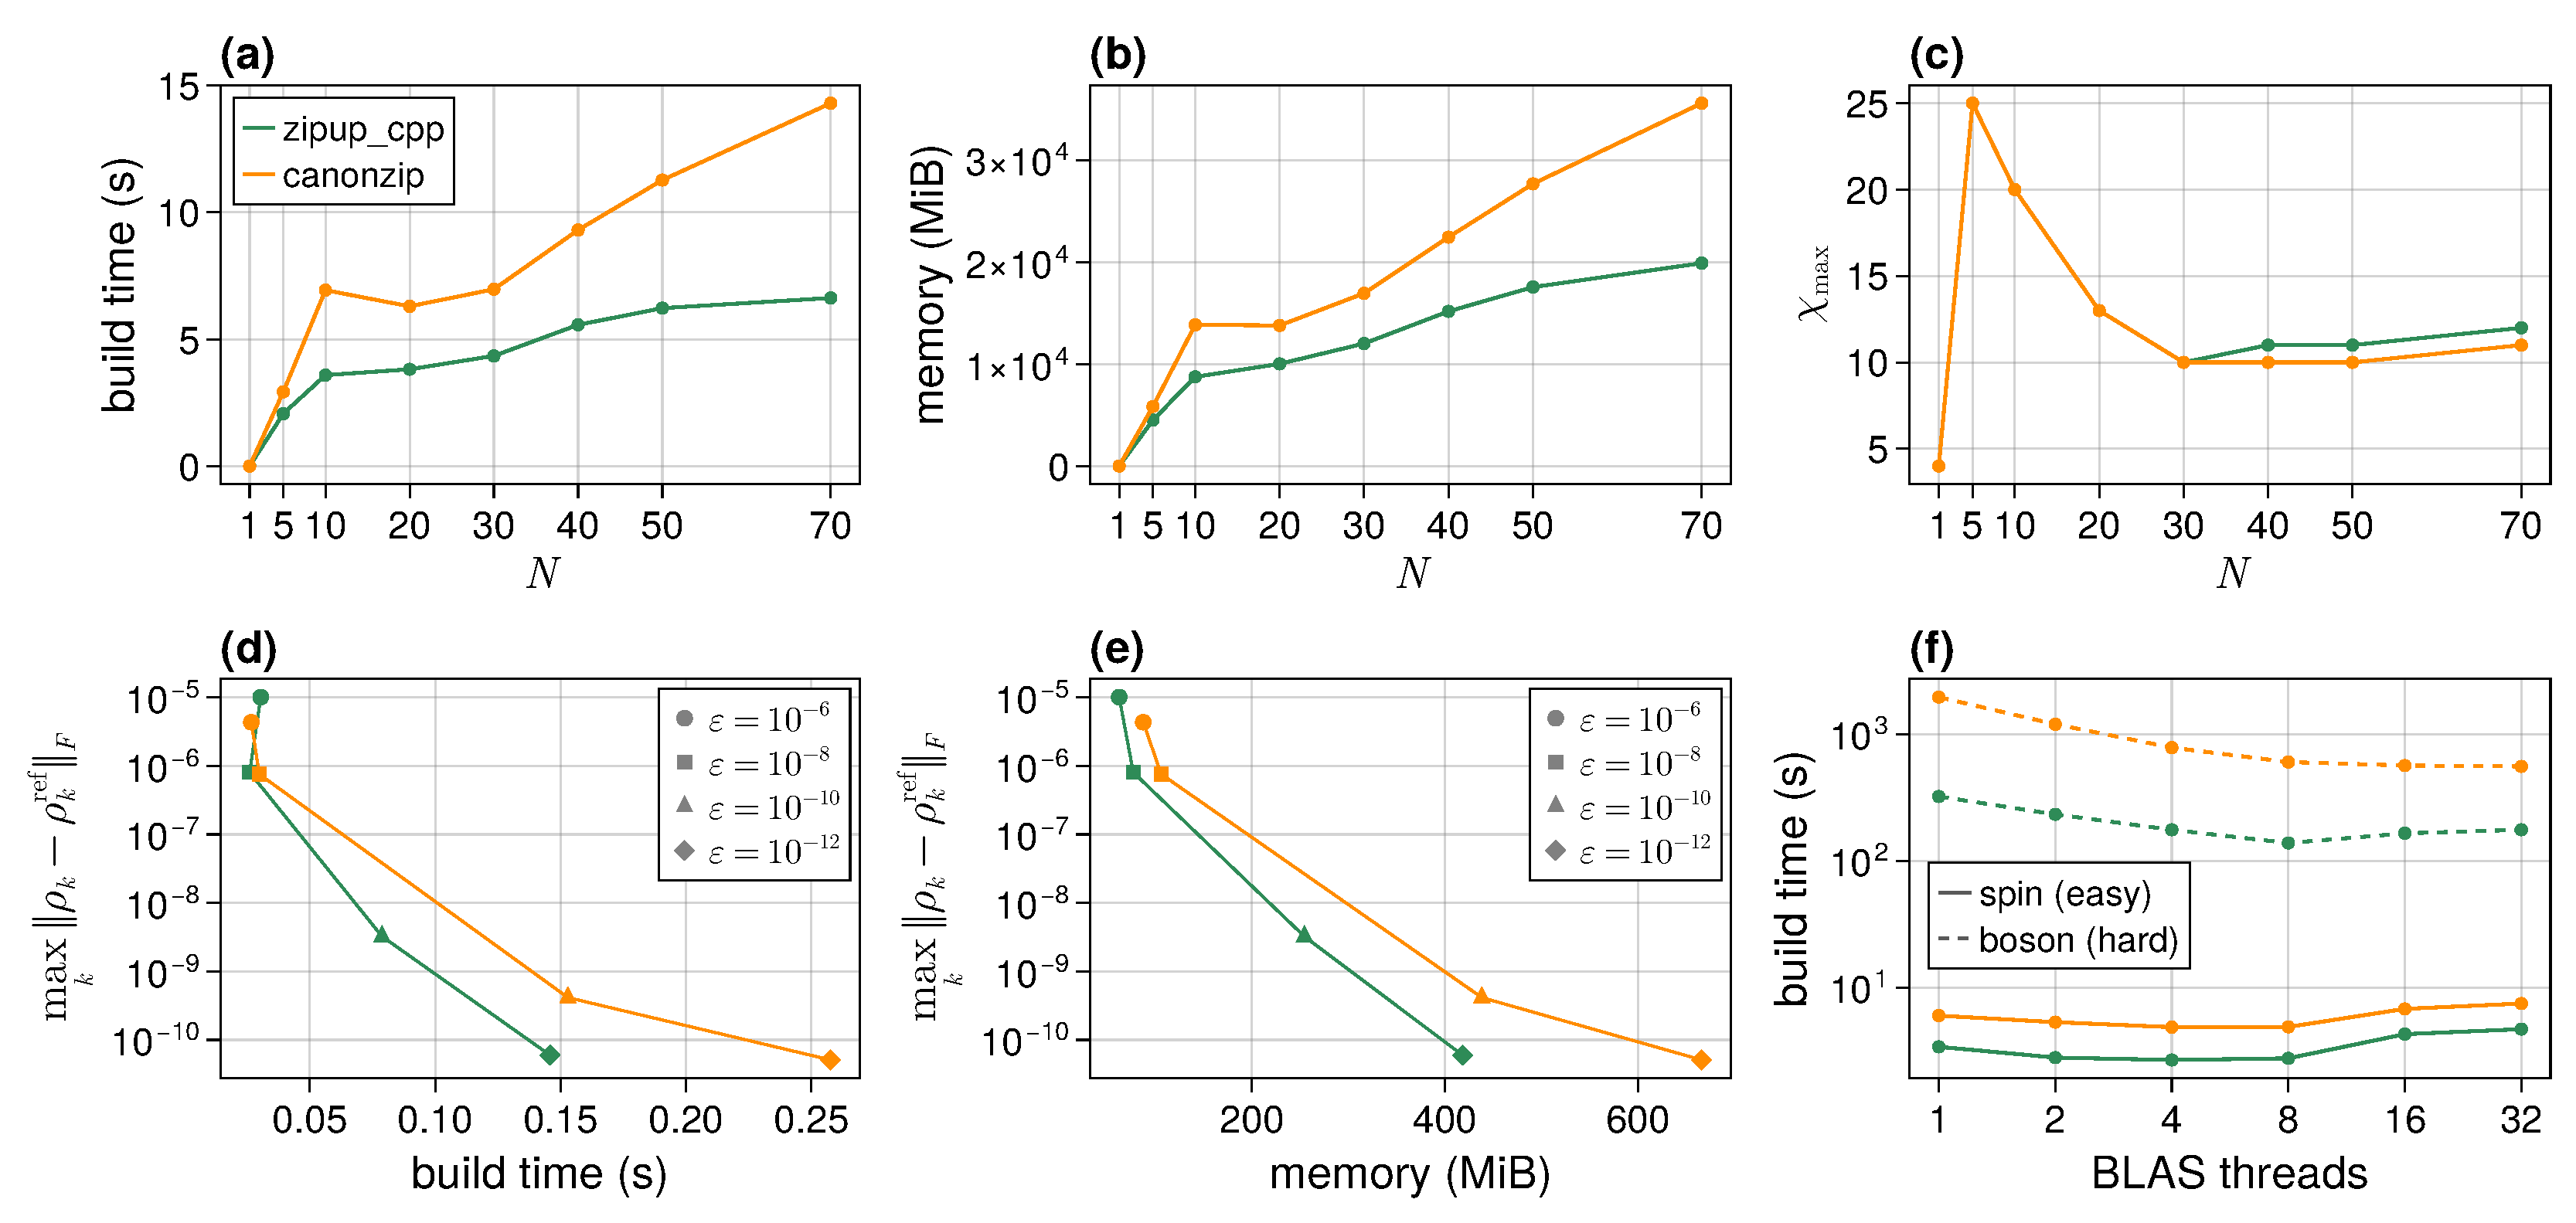
\includegraphics[width=0.98\textwidth]{figures/ace_compression.pdf}
    \caption{Comparison of the two ACE compression schedules.
    Panels (a)--(c) show median build time, total allocated memory, and maximum temporal bond dimension of the two compression schedules for the unpolarised central-spin scaling, benchmarked over seven samples.
    Panels (d)--(e) show trajectory error relative to a tightly converged reference.
    Panel (f) shows one benchmarked build per BLAS thread count for fixed spin (easy) and bosonic (hard) process tensors.}
    \label{fig:ace-compressors}
\end{figure*}
%

Figure~\ref{fig:ace-compressors} compares these schedules.
Panels (a) and (b) show that \texttt{:zipup\_cpp} is consistently faster and allocates less memory than \texttt{:canonzip} as the spin bath grows.
This saving does not come from retaining a smaller final PT-MPO: panel (c) shows comparable bond dimensions, with \texttt{:canonzip} sometimes reaching a slightly smaller \(\chi_{\max}\).
The benefit of canonicalisation is clearest in panels (d) and (e).
At each matched cutoff, \texttt{:canonzip} produces the smaller trajectory error, so it is the more accurate compression schedule for a fixed truncation threshold, but that accuracy is purchased with greater runtime and memory allocation.

Panel (f) isolates parallelism that can be used inside the SVDs by varying the BLAS thread count.
ITensors uses LAPACK's divide-and-conquer \texttt{gesdd} routine for these decompositions, so users can accelerate sufficiently large ACE builds through a multithreaded BLAS/LAPACK backend.
The ``easy'' case is a five-mode polarised spin bath with local Hilbert dimension \(2\), \(200\) time steps, cutoff \(10^{-10}\), and \(\chi_{\max}=28\).
The ``hard'' case is an eight-mode Lorentzian bosonic bath with local dimension \(5\), \(60\) time steps, cutoff \(10^{-8}\), and \(\chi_{\max}\simeq50\).
Its larger mode indices and temporal bonds produce much larger SVD matrices, making the build more expensive while exposing enough dense linear-algebra work for effective BLAS parallelism.
For the smaller spin problem, the SVD matrices are too small to pay for the overhead of thread-startup, scheduling, and synchronization, so additional BLAS threads provide little benefit and can even increase runtime.
In the bosonic case, large SVDs dominate the build and their BLAS kernels contain sufficient parallel work to produce substantial speedup.

The relative merits of canonicalising before truncation and truncating during the forward zip-up sweep were raised in Referee Report~1 and the accompanying author response in the SciPost submission thread~\cite{SciPostReport9135}.
The referee argued that canonicalising before truncation makes each SVD locally optimal, while the authors defended forward truncation as a substantially faster approximation that remains accurate in practice.
Our results in Fig.~\ref{fig:ace-compressors} indeed show a trade-off rather than a universally superior schedule: \texttt{:canonzip} is more accurate at a fixed cutoff, whereas \texttt{:zipup\_cpp} is faster and uses less memory.
A tighter zip-up cutoff can recover the required accuracy, so the appropriate choice depends on the available memory and target error.

%%%%%%%%%%%%%%%%%%%%%%%%%%%%%%%%%%%%%%%%%%%%%%%%%%%%%%%%%%%%%%%%%%%%%%%%%%%
\subsection{Benchmark against the original C++ ACE toolkit}
\label{subsec:ace-cpp-comparison}

We finally compare \texttt{ProcessTensors.jl} with the original C++ ACE toolkit of Cygorek and Gauger~\cite{CygorekGauger2024}, available from its public source repository.\footnote{\url{https://github.com/mcygorek/ACE}}
For both Julia and C++, BLAS, MKL, and OpenMP were restricted to one thread and independent cases were pinned to separate CPUs.
Julia was warmed before timing to ignore compilation time; C++ was compiled with \texttt{-O3} and Eigen.
Versions, compiler flags, affinity, thread counts, and model parameters are recorded in the metadata of the runs.

The benchmark covers fully polarised, partially polarised, and unpolarised central-spin baths, together with a Lorentzian spin--boson bath,
%
\begin{equation}
    J(\omega)=\frac{C}{\pi}\frac{\gamma}{(\omega-\omega_c)^2+\gamma^2},
    \qquad \omega_c=\Omega,\quad\gamma=0.1\Omega ,
    \label{eq:ace-lorentzian}
\end{equation}
%
with \(C/\Omega^2=0.2\), \(M=5\), \(\Omega T=8\), \(\Omega\Delta t=0.1\), and \(k_BT/\Omega\in\{0,0.5,1,3\}\).
Both implementations use the same timestep, final time, bath discretisation, relative cutoff, second-order propagation choice, and bath realisation.
For the partially polarised and unpolarised central-spin cases, the bath-spin orientations generated by C++ are read back and supplied directly to our Julia constructors.

%
\begin{figure*}[h]
    \centering
    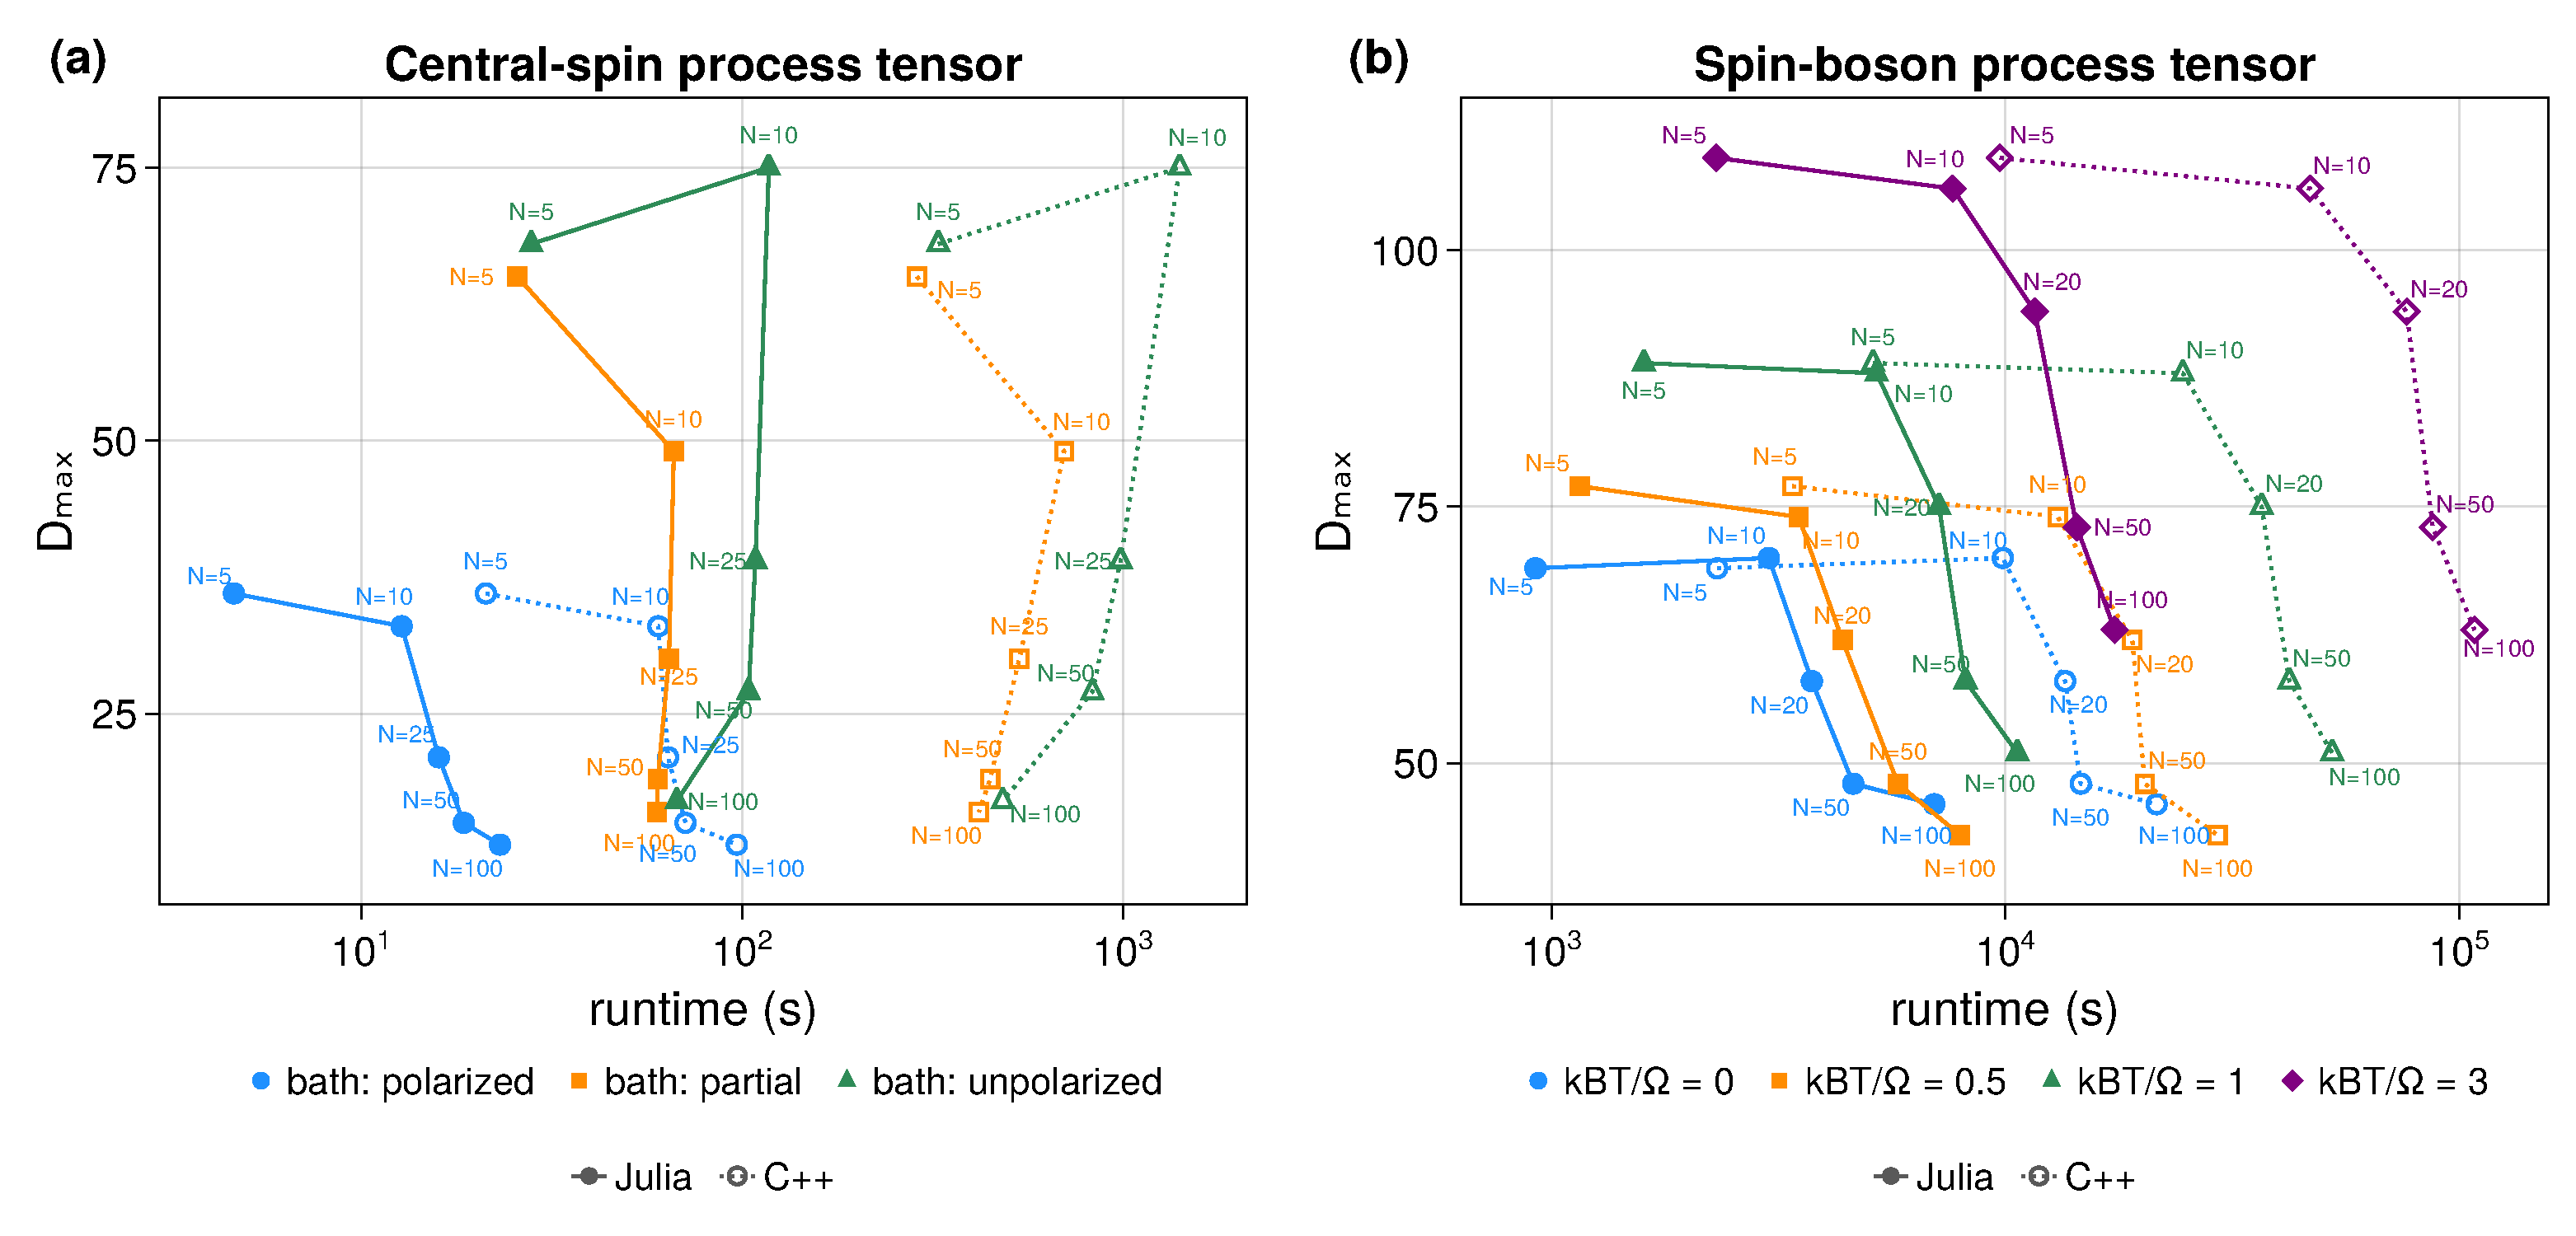
\includegraphics[width=0.98\textwidth]{figures/ace_julia_vs_cpp.pdf}
    \caption{Benchmark of \texttt{ProcessTensors.jl} against the original C++ ACE toolkit.
    (a) Central-spin baths with fully polarised, partially polarised, and unpolarised initial states.
    (b) Lorentzian spin--boson baths at four different temperatures.
    Filled symbols denote Julia and open symbols C++; labels give the number \(N\) of bath modes.
    The horizontal axis is measured PT-MPO construction time and the vertical axis is the maximum internal bond dimension \(D_{\max}\).
    Vertical alignment of matched points indicates equal retained bond dimension.}
    \label{fig:ace-cpp}
\end{figure*}
%

Figure~\ref{fig:ace-cpp} compares construction time and \(D_{\max}\) as the number of bath modes is increased for three central-spin polarisations [panel (a)] and four spin--boson temperatures [panel (b)].

Across both model families, matched Julia and C++ points have the same \(D_{\max}\), showing that the two implementations retain the same maximum temporal complexity under the matched cutoff and propagation settings.
The Julia points lie consistently to the left of their C++ counterparts, corresponding to faster construction times for every tested bath size, polarisation, and temperature.
The Julia path uses the ITensors LAPACK divide-and-conquer SVD, whereas the C++ implementation uses Eigen's JacobiSVD; contraction order, tensor permutation, allocation, and serialization also differ.
The comparison therefore demonstrates matched compression and the end-to-end performance obtained by the present workflows to construct the process tensor.

Together these benchmarks establish the hierarchy of controls that should be reported in practical ACE calculations: the timestep and Trotter order determine propagation error; the bath grid determines which environmental correlations are represented; the SVD cutoff and \texttt{maxdim} determine how much of that representation is retained; and the compression schedule determines the intermediate cost.
